% Created 2024-10-18 vie 19:17
% Intended LaTeX compiler: pdflatex
\documentclass[10pt]{article}
\usepackage[utf8]{inputenc}
\usepackage{lmodern}
\usepackage[T1]{fontenc}
\usepackage[top=1in, bottom=1.in, left=1in, right=1in]{geometry}
\usepackage{graphicx}
\usepackage{longtable}
\usepackage{float}
\usepackage{wrapfig}
\usepackage{rotating}
\usepackage[normalem]{ulem}
\usepackage{amsmath}
\usepackage{textcomp}
\usepackage{marvosym}
\usepackage{wasysym}
\usepackage{amssymb}
\usepackage{amsmath}
\usepackage[theorems, skins]{tcolorbox}
\usepackage[version=3]{mhchem}
\usepackage[numbers,super,sort&compress]{natbib}
\usepackage{natmove}
\usepackage{url}
\usepackage[cache=false]{minted}
\usepackage[strings]{underscore}
\usepackage[linktocpage,pdfstartview=FitH,colorlinks,
linkcolor=blue,anchorcolor=blue,
citecolor=blue,filecolor=blue,menucolor=blue,urlcolor=blue]{hyperref}
\usepackage{attachfile}
\usepackage{setspace}
\usepackage[spanish, ]{babel}
\date{}
\title{Segundo ejercicio de identificación de un modelo ARIMA}
\begin{document}

\maketitle
\section*{Datos}
\label{sec:org4e7af39}

Cargue la serie de datos simulados \href{IdentificaEstosARIMA/00c296-12.gdt}{00c296-12.gdt}

\begin{minted}[frame=lines,fontsize=\scriptsize,linenos=]{r}
open IdentificaEstosARIMA/00c296-12.gdt
\end{minted}
\subsection*{Tareas a realizar}
\label{sec:org3fae9e9}

\begin{enumerate}
\item \hyperref[sec:org6c88b85]{Realice un primer análisis gráfico: haga
un gráfico de la serie y un gráfico \emph{rango-media}}
\item \hyperref[sec:org6142ddf]{Determine si es necesario transformar logarítmicamente los datos}
\item \hyperref[sec:orgd530ff7]{Determine si es necesario tomar una
diferencia estacional de la serie}
\item \hyperref[sec:orgc98824b]{Determine si es necesario tomar una o
más diferencias regulares de la serie}
\item \hyperref[sec:org459f8d2]{Encuentre un modelo ARIMA para la
serie que sea lo más parsimonioso posible, pero cuyos residuos se
puedan considerar \emph{ruido blanco}.}
\end{enumerate}
\section*{Primer análisis gráfico}
\label{sec:org6c88b85}


\begin{minted}[frame=lines,fontsize=\scriptsize,linenos=]{r}
gnuplot x --time-series --with-lines --output="SerieEnNiveles.png"
rmplot  x --output="rango-media.png"
\end{minted}

\begin{center}
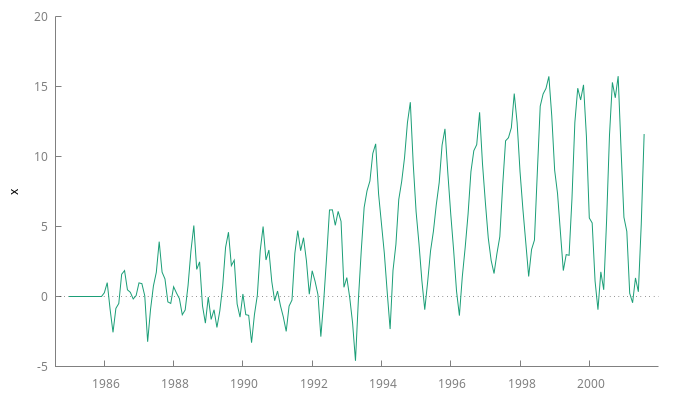
\includegraphics[width=0.5\textwidth]{./SegundoEjercicioIdentificacionModeloARIMA/SerieEnNiveles.png}
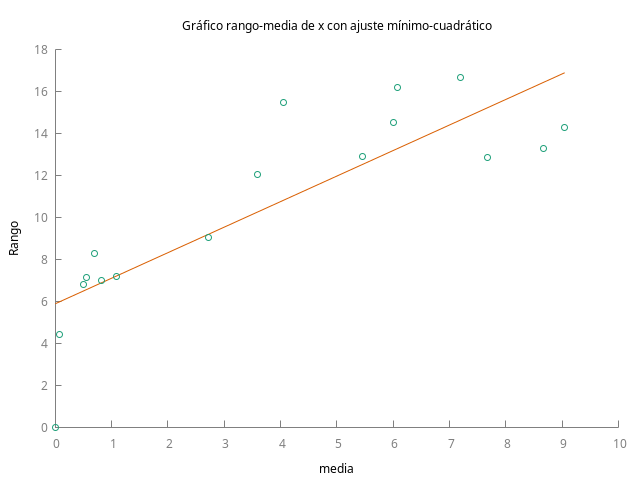
\includegraphics[width=0.4\textwidth]{./SegundoEjercicioIdentificacionModeloARIMA/rango-media.png} 
\end{center}

De estos gráficos se desprende que la serie tiene una acusada pauta
estacional y que la volatilidad probablemente depende del nivel de la
serie.
\section*{Estacionariedad en varianza}
\label{sec:org6142ddf}

A la luz de los anteriores gráficos, donde se aprecia que la
variabilidad de los datos aumenta con el nivel de la serie, parece
necesaria la transformación logarítmica; pero esta serie toma valores
negativos, por lo que \textbf{no podemos transformar los datos
logarítmicamente} (para hacerlo deberíamos sumar previamente un valor
constante suficientemente elevado como para que todos los valores
fueran positivos). Por el momento, dejemos la serie sin transformarla
logarítmicamente.
\section*{Diferencias estacionales}
\label{sec:orgd530ff7}

Observemos el gráfico de la serie y su correlograma.

\begin{minted}[frame=lines,fontsize=\scriptsize,linenos=]{r}
corrgm x 36 --plot="x_ACF-PACF.png"
\end{minted}


\begin{center}
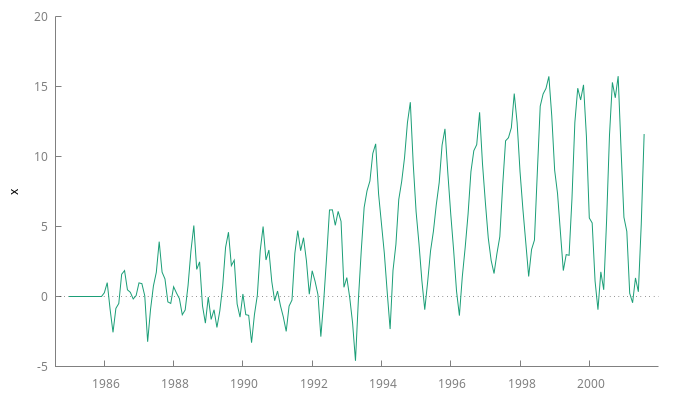
\includegraphics[width=0.5\textwidth]{./SegundoEjercicioIdentificacionModeloARIMA/SerieEnNiveles.png}
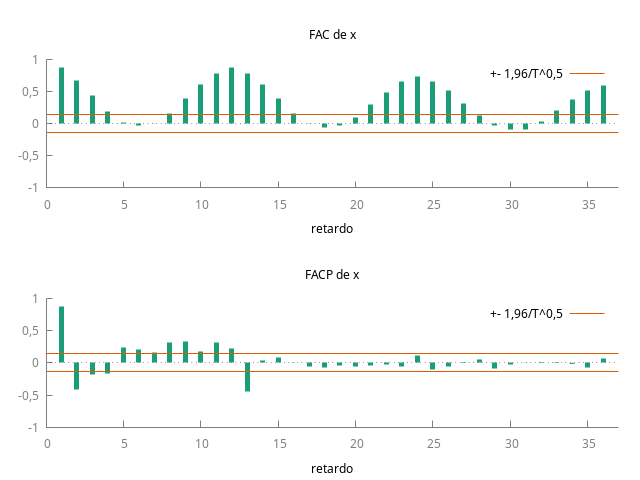
\includegraphics[width=0.5\textwidth]{./SegundoEjercicioIdentificacionModeloARIMA/x_ACF-PACF.png}
\end{center}

En el gráfico de la serie se aprecia una acusada pauta estacional. En
la función de autocorrelación simple las correlaciones
correspondientes a los retardos estacionales son muy significativas (y
con bastantes ``satélites''); en la función de autocorrelación parcial
los 13 primeros retardos son muy significativos, en particular, el
decimotercero (adyacente al 12) es muy importante.

Además, si tratamos de ajustar un AR(1) estacional:

\begin{minted}[frame=lines,fontsize=\scriptsize,linenos=]{r}
ARIMA000X100 <- arima 0 0 0 ; 1 0 0 ; x 
\end{minted}

\begin{verbatim}
Evaluaciones de la función: 622
Evaluaciones del gradiente: 123

ARIMA000X100:
ARMA, usando las observaciones 1985:01-2001:08 (T = 200)
Estimado usando AS 197 (MV exacta)
Variable dependiente: x
Desviaciones típicas basadas en el Hessiano

             coeficiente   Desv. típica     z      valor p
  --------------------------------------------------------
  const       3,59533       1,28683        2,794   0,0052  ***
  Phi_1       0,955320      0,0148914     64,15    0,0000  ***

Media de la vble. dep.  3,780099   D.T. de la vble. dep.   4,838896
Media de innovaciones   0,358041   D.T. innovaciones       1,535258
R-cuadrado              0,906552   R-cuadrado corregido    0,906552
Log-verosimilitud      −384,1534   Criterio de Akaike      774,3069
Criterio de Schwarz     784,2019   Crit. de Hannan-Quinn   778,3112

                       Real Imaginaria     Módulo Frecuencia
  -----------------------------------------------------------
  AR (estacional)
   Raíz  1           1,0468     0,0000     1,0468     0,0000
  -----------------------------------------------------------

ARIMA000X100 guardado
\end{verbatim}

constatamos que la estimación del parámetro \(\Phi_1\) está muy próxima a uno.

\textbf{Estas evidencias apuntan a que es necesario tomar una diferencia
estacional}

Recuerde que los test ADF y KPSS no sirven para determinar si es
necesario tomar diferencias estacionales (solo sirven para las
diferencias regulares).

Por tanto, tomamos una diferencia estacional.

\begin{minted}[frame=lines,fontsize=\scriptsize,linenos=]{r}
sdiff x
gnuplot sd_x --time-series --with-lines --output="SerieEnDiferencias.png"
\end{minted}

\begin{center}
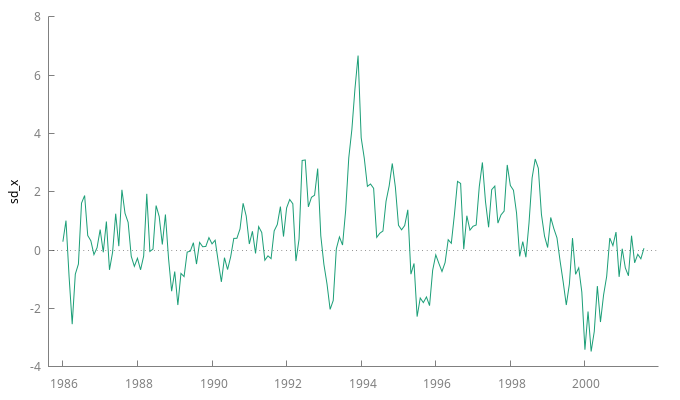
\includegraphics[width=0.5\textwidth]{./SegundoEjercicioIdentificacionModeloARIMA/SerieEnDiferencias.png}
\end{center}
\subsection*{Repetición del análisis con la serie diferenciada estacionalmente}
\label{sec:orgee64740}


La serie resultante no muestra signos de estacionalidad. Veamos si se
ve algo en el correlograma:

\begin{minted}[frame=lines,fontsize=\scriptsize,linenos=]{r}
corrgm sd_x 36 --plot="sd_x_ACF-PACF.png"
\end{minted}


\begin{center}
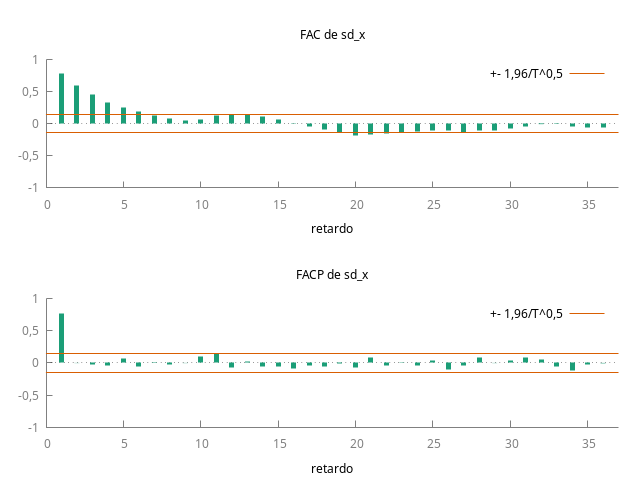
\includegraphics[width=0.5\textwidth]{./SegundoEjercicioIdentificacionModeloARIMA/sd_x_ACF-PACF.png}
\end{center}

\textbf{No hay nada que sugiera la necesidad de tomar una segunda diferencia
estacional}.
\section*{Estacionariedad en media}
\label{sec:orgc98824b}

El gráfico de la serie diferenciada estacionalmente no muestra tener
una clara tendencia o evolución a largo plazo de su nivel.


\begin{center}
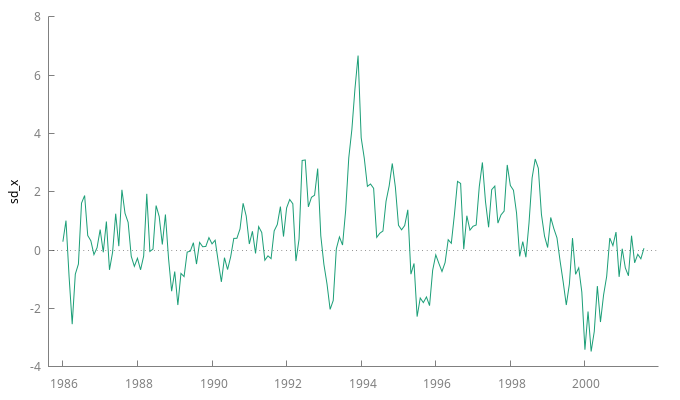
\includegraphics[width=0.5\textwidth]{./SegundoEjercicioIdentificacionModeloARIMA/SerieEnDiferencias.png}
\end{center}

En el correlograma, la ACF decae rápidamente, indicando que la serie
parece ser la realización de un proceso estacionario.

\begin{center}
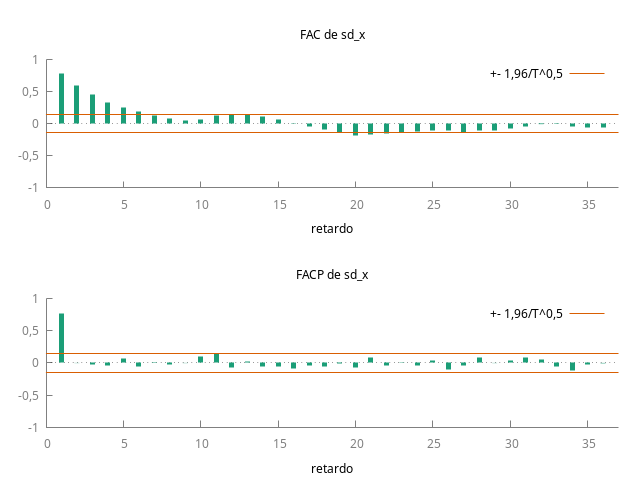
\includegraphics[width=0.5\textwidth]{./SegundoEjercicioIdentificacionModeloARIMA/sd_x_ACF-PACF.png}
\end{center}

Probemos a ajustar un modelo AR a los datos diferenciados estacionalmente

\begin{minted}[frame=lines,fontsize=\scriptsize,linenos=]{r}
ARIMA110 <- arima 1 1 0 ; x
\end{minted}

\begin{verbatim}
Evaluaciones de la función: 20
Evaluaciones del gradiente: 5

ARIMA110: ARIMA, usando las observaciones 1985:02-2001:08 (T = 199)
Estimado usando AS 197 (MV exacta)
Variable dependiente: (1-L) x
Desviaciones típicas basadas en el Hessiano

             coeficiente   Desv. típica     z      valor p 
  ---------------------------------------------------------
  const       0,0799826     0,255554      0,3130   0,7543  
  phi_1       0,405536      0,0659820     6,146    7,94e-10 ***

Media de la vble. dep.  0,058438   D.T. de la vble. dep.   2,351529
Media de innovaciones   0,000197   D.T. innovaciones       2,149835
R-cuadrado              0,824333   R-cuadrado corregido    0,824333
Log-verosimilitud      −434,7714   Criterio de Akaike      875,5428
Criterio de Schwarz     885,4227   Crit. de Hannan-Quinn   879,5415

                       Real Imaginaria     Módulo Frecuencia
  -----------------------------------------------------------
  AR
   Raíz  1           2,4659     0,0000     2,4659     0,0000
  -----------------------------------------------------------

ARIMA110 guardado
\end{verbatim}

El parámetro \(\phi_1\) está muy lejos de la unidad (consecuentemente,
también lo está la raíz autorregresiva).

Probemos con los tests formales de raíz unitaria y estacionariedad
\subsubsection*{Test ADF}
\label{sec:org83999fe}

\begin{minted}[frame=lines,fontsize=\scriptsize,linenos=]{r}
adf -1 sd_x --c --gls --test-down --perron-qu 
\end{minted}

\begin{verbatim}
Contraste aumentado de Dickey-Fuller (GLS) para sd_x
contrastar hacia abajo desde 14 retardos, con el criterio AIC modificado, Perron-Qu
tamaño muestral 187
la hipótesis nula de raíz unitaria es: [a = 1]

  contraste con constante 
  incluyendo 0 retardos de (1-L)sd_x
  modelo: (1-L)y = b0 + (a-1)*y(-1) + e
  valor estimado de (a - 1): -0,225392
  estadístico de contraste: tau = -4,85952
  valor p aproximado 0,000
  Coef. de autocorrelación de primer orden de e: 0,002
\end{verbatim}

El p-valores es muy bajo, por lo que se rechaza la \(H_0\) de que la serie es \(I(1)\)
\subsubsection*{Test KPSS}
\label{sec:org87566bf}

\begin{minted}[frame=lines,fontsize=\scriptsize,linenos=]{r}
kpss -1 sd_x 
\end{minted}

\begin{verbatim}
Contraste KPSS para sd_x

T = 188
Parámetro de truncamiento de los retardos = 4
Estadístico de contraste = 0,22692

                      10%      5%      1%
Valores críticos: 0,348   0,462   0,739
Valor p > .10
\end{verbatim}

El p-valor es elevado, por los que NO se rechaza la \(H_0\) de que la
serie es \(I(0)\). \textbf{Todas estas evidencias indican de manera muy clara
que NO es necesario tomar ninguna diferencia ordinaria}.
\section*{Primer intento de búsqueda de un modelo ARIMA}
\label{sec:org459f8d2}

Observando al ACF y la PACF de aprecia que la ACF decae a una tasa
exponencial, y la PACF se trunca tras el primer retardo, lo cual es
compatible con un AR(1).

\begin{center}
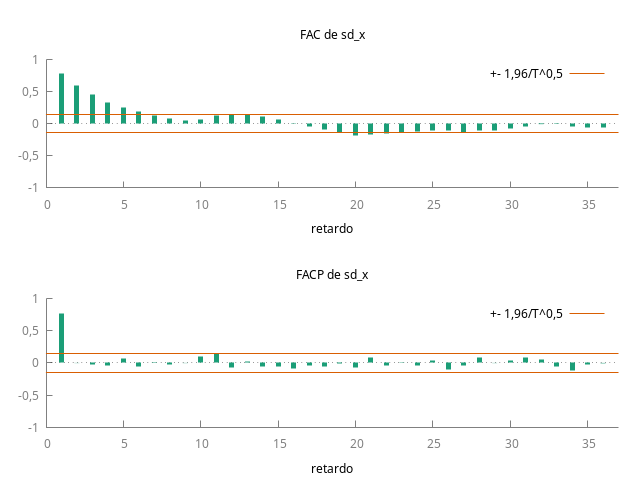
\includegraphics[width=0.5\textwidth]{./SegundoEjercicioIdentificacionModeloARIMA/sd_x_ACF-PACF.png}
\end{center}

Por tanto, parece que la serie en logaritmos sigue un modelo
ARIMA\((1,1,0)\). Veamos si es así:

\begin{minted}[frame=lines,fontsize=\scriptsize,linenos=]{r}
ARIMA110cte <- arima 1 1 0 ; x 
\end{minted}

\begin{verbatim}
Evaluaciones de la función: 20
Evaluaciones del gradiente: 5

ARIMA110cte:
ARIMA, usando las observaciones 1985:02-2001:08 (T = 199)
Estimado usando AS 197 (MV exacta)
Variable dependiente: (1-L) x
Desviaciones típicas basadas en el Hessiano

             coeficiente   Desv. típica     z      valor p 
  ---------------------------------------------------------
  const       0,0799826     0,255554      0,3130   0,7543  
  phi_1       0,405536      0,0659820     6,146    7,94e-10 ***

Media de la vble. dep.  0,058438   D.T. de la vble. dep.   2,351529
Media de innovaciones   0,000197   D.T. innovaciones       2,149835
R-cuadrado              0,824333   R-cuadrado corregido    0,824333
Log-verosimilitud      −434,7714   Criterio de Akaike      875,5428
Criterio de Schwarz     885,4227   Crit. de Hannan-Quinn   879,5415

                       Real Imaginaria     Módulo Frecuencia
  -----------------------------------------------------------
  AR
   Raíz  1           2,4659     0,0000     2,4659     0,0000
  -----------------------------------------------------------

ARIMA110cte guardado
\end{verbatim}

Los parámetros autorregresivos son significativos y el modulo de las
raíces es claramente mayor que la unidad en ambos casos. No obstante,
la constante no es significativa. 

Reestimemos el modelo sin constante:

\begin{minted}[frame=lines,fontsize=\scriptsize,linenos=]{r}
ARIMA110 <- arima 1 0 0; 0 1 0 ; x --nc
\end{minted}

\begin{verbatim}
Evaluaciones de la función: 16
Evaluaciones del gradiente: 3

ARIMA110: ARIMA, usando las observaciones 1986:01-2001:08 (T = 188)
Estimado usando AS 197 (MV exacta)
Variable dependiente: (1-Ls) x
Desviaciones típicas basadas en el Hessiano

             coeficiente   Desv. típica     z     valor p 
  --------------------------------------------------------
  phi_1       0,787833      0,0440563     17,88   1,62e-71 ***

Media de la vble. dep.  0,449786   D.T. de la vble. dep.   1,487227
Media de innovaciones   0,095115   D.T. innovaciones       0,946555
R-cuadrado              0,962771   R-cuadrado corregido    0,962771
Log-verosimilitud      −256,9190   Criterio de Akaike      517,8381
Criterio de Schwarz     524,3110   Crit. de Hannan-Quinn   520,4606

                       Real Imaginaria     Módulo Frecuencia
  -----------------------------------------------------------
  AR
   Raíz  1           1,2693     0,0000     1,2693     0,0000
  -----------------------------------------------------------

ARIMA110 guardado
\end{verbatim}
\subsection*{Análisis de los residuos}
\label{sec:org8297dd5}

Todo parece OK, pero debemos ver el gráfico de los residuos y su
correlograma, así como los estadísticos Q de Ljung-Box para constatar
si podemos asumir que son la realización de un proceso de ruido
blanco.

\begin{minted}[frame=lines,fontsize=\scriptsize,linenos=]{r}
series residuos = $uhat
\end{minted}

\begin{minted}[frame=lines,fontsize=\scriptsize,linenos=]{r}
gnuplot residuos --time-series --with-lines --output="Residuos.png"
corrgm residuos 60 --plot="residuosACF-PACF.png"
\end{minted}

\begin{center}
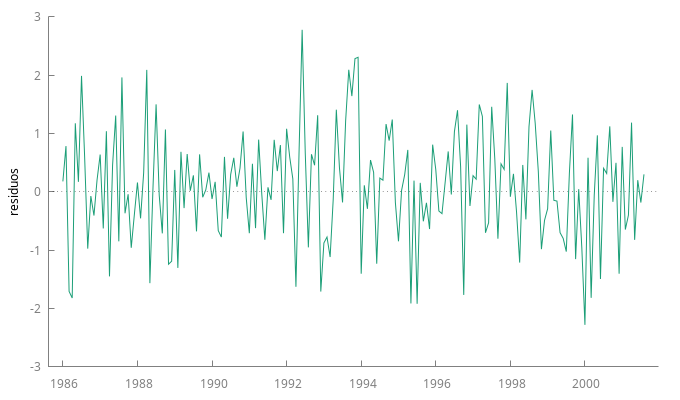
\includegraphics[width=0.5\textwidth]{./SegundoEjercicioIdentificacionModeloARIMA/Residuos.png}
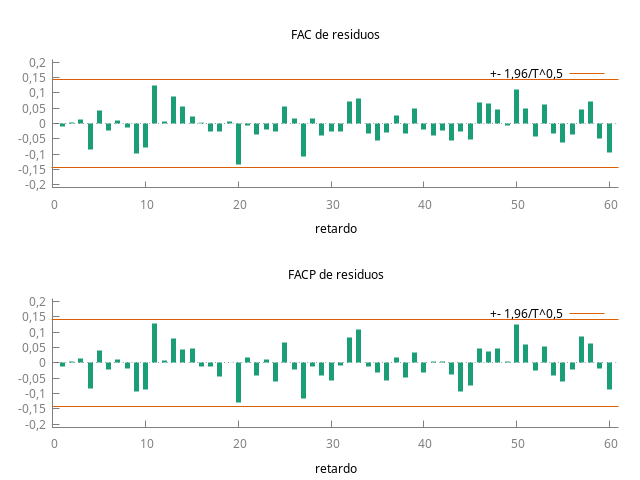
\includegraphics[width=0.5\textwidth]{./SegundoEjercicioIdentificacionModeloARIMA/residuosACF-PACF.png}
\end{center}

\begin{minted}[frame=lines,fontsize=\scriptsize,linenos=]{r}
corrgm residuos 15
\end{minted}


\begin{verbatim}
Función de autocorrelación para residuos
***, ** y * indica significatividad a los niveles del 1%, 5% y 10%
utilizando la desviación típica 1/T^0,5

 RETARDO    FAC          FACP         Estad-Q. [valor p]

    1  -0,0117       -0,0117          0,0260  [0,872]
    2   0,0043        0,0042          0,0296  [0,985]
    3   0,0141        0,0142          0,0677  [0,995]
    4  -0,0841       -0,0838          1,4398  [0,837]
    5   0,0410        0,0393          1,7673  [0,880]
    6  -0,0229       -0,0218          1,8703  [0,931]
    7   0,0091        0,0108          1,8867  [0,966]
    8  -0,0119       -0,0199          1,9146  [0,984]
    9  -0,0982       -0,0921          3,8399  [0,922]
   10  -0,0798       -0,0882          5,1169  [0,883]
   11   0,1237  *     0,1294 *        8,2065  [0,695]
   12   0,0056        0,0074          8,2128  [0,768]
   13   0,0892        0,0790          9,8375  [0,707]
   14   0,0536        0,0451         10,4283  [0,730]
   15   0,0221        0,0466         10,5290  [0,785]
\end{verbatim}

El gráfico de los residuos no presenta ninguna estructura reconocible
y ninguna autocorrelación es significativa.

Más importante aún, \textbf{los correlogramas no muestran ninguna pauta
reconocible, se parecen mucho entre sí y los estadísticos Q muestran
p-valores muy elevados}, por lo que podemos asumir que estos residuos
son ``ruido blanco''.
\medskip

También conviene mirar si los residuos tienen distribución gaussiana:
\medskip

\begin{minted}[frame=lines,fontsize=\scriptsize,linenos=]{r}
modtest --normality
\end{minted}

\begin{verbatim}
Distribución de frecuencias para uhat8, observaciones 13-200
número de cajas = 13, Media = 0,0951153, Desv.típ.=0,944279

      intervalo     punto medio   frecuencia  rel     acum.

           < -2,0695   -2,2803        1      0,53%    0,53% 
   -2,0695 - -1,6480   -1,8588        7      3,72%    4,26% *
   -1,6480 - -1,2265   -1,4373        9      4,79%    9,04% *
   -1,2265 - -0,80505  -1,0158       15      7,98%   17,02% **
  -0,80505 - -0,38355  -0,59430      24     12,77%   29,79% ****
  -0,38355 -  0,037942 -0,17281      30     15,96%   45,74% *****
  0,037942 -  0,45944   0,24869      39     20,74%   66,49% *******
   0,45944 -  0,88094   0,67019      26     13,83%   80,32% ****
   0,88094 -  1,3024    1,0917       19     10,11%   90,43% ***
    1,3024 -  1,7239    1,5132        9      4,79%   95,21% *
    1,7239 -  2,1454    1,9347        6      3,19%   98,40% *
    2,1454 -  2,5669    2,3562        2      1,06%   99,47% 
          >=  2,5669    2,7777        1      0,53%  100,00% 

Contraste de la hipótesis nula de distribución Normal:
Chi-cuadrado(2) = 0,023 con valor p 0,98858
\end{verbatim}

Claramente tienen distribución normal.


Si en la ventana del modelo estimado pincha en el menú
desplegable \texttt{Gráficos -{}-{}> Espectro con respecto al periodograma
espectral} verá que el espectro teórico del modelo se ajusta
perfectamente al periodograma de la serie.
\medskip

Por tanto, podemos concluir que la serie \texttt{00c296-12.gdt}, no requiere
la transformación logarítmica (en cualquier caso no se podía tomar sin
aumentar previamente su nivel para hacerla positiva), sigue un proceso
ARIMA\((1,0,0)\times(0,1,0)_S\) con media cero.
\subsection*{Modelo efectivamente simulado}
\label{sec:orgefc5d4d}

Veamos si ese es el modelo usado en su simulación. Si miramos la línea
\texttt{150} del fichero \href{IdentificaEstosARIMA/000-Etiquetas-12.txt}{000-Etiquetas-12.txt} que se encuentra en el directorio de
donde hemos obtenido los datos encontramos lo siguiente:
\medskip

\begin{center}
\begin{tabular}{l}
\texttt{00c296,	    ,	mu = 0.0,	ar = '(1 - 0.8B)(1 + 0.8B)', ma = '(1 + 0.55B)', i = '(1 - B12)'}\\
\end{tabular}
\end{center}

\medskip

Efectivamente, NO requería la transformación logarítmica, la media era
\(0.0\) y era necesaria una diferencia estacional, pero ninguna regular.

No obstante, el modelo simulado tenía un polinomio autorregresivo de
de orden dos, AR(2), y un polinomio de media móvil de orden uno,
MA(1). Veamos qué pasa si intentamos estimar el verdadero modelo
simulado\ldots{}

\textbf{¡Hemos identificado un modelo distinto del simulado!}
\section*{Pruebas con otro modelo ARIMA}
\label{sec:org22fc477}

Estimemos el verdadero modelo ARIMA\((2,0,0)\times(1,1,0)_{S}\):

\begin{minted}[frame=lines,fontsize=\scriptsize,linenos=]{r}
ARIMAsimulado <- arima 2 0 0; 1 1 0 ; x --nc
\end{minted}

\begin{verbatim}
Evaluaciones de la función: 27
Evaluaciones del gradiente: 7

ARIMAsimulado:
ARIMA, usando las observaciones 1986:01-2001:08 (T = 188)
Estimado usando AS 197 (MV exacta)
Variable dependiente: (1-Ls) x
Desviaciones típicas basadas en el Hessiano

             coeficiente   Desv. típica      z      valor p 
  ----------------------------------------------------------
  phi_1       0,777533      0,0747739     10,40     2,52e-25 ***
  phi_2       0,0107529     0,0738538      0,1456   0,8842  
  Phi_1       0,0187954     0,0773800      0,2429   0,8081  

Media de la vble. dep.  0,449786   D.T. de la vble. dep.   1,487227
Media de innovaciones   0,093115   D.T. innovaciones       0,946381
R-cuadrado              0,962765   R-cuadrado corregido    0,962363
Log-verosimilitud      −256,8841   Criterio de Akaike      521,7682
Criterio de Schwarz     534,7139   Crit. de Hannan-Quinn   527,0133

                       Real Imaginaria     Módulo Frecuencia
  -----------------------------------------------------------
  AR
   Raíz  1           1,2640     0,0000     1,2640     0,0000
   Raíz  2         -73,5729     0,0000    73,5729     0,5000
  AR (estacional)
   Raíz  1          53,2046     0,0000    53,2046     0,0000
  -----------------------------------------------------------

ARIMAsimulado guardado
\end{verbatim}

El ajuste es parecido (fíjese en los coeficientes de determinación)
pero solo el parámetro \(\phi_1\) resulta ser significativo (y con un
valor parecido al del modelo anterior). Por tanto\ldots{}
\bigskip

La estimación del verdadero modelo empleado en la simulación de los
datos ¡NO ES MEJOR QUE EL MODELO QUE HEMOS IDENTIFICADO!

La explicación es que el factor \((1 + 0.8\mathsf{B})\) del polinomio AR
casi se cancela con el polinomio MA \(\;(1 + 0.55\mathsf{B})\). Por eso hemos encontrado un modelo más parsimonioso que funciona OK.
\bigskip


\textbf{\uline{Ahora escoja al azar nuevas series del \href{https://github.com/mbujosab/EconometriaAplicada-SRC/tree/main/Ejercicios/IdentificaEstosARIMA}{directorio} (dispone de
 centenares de series simuladas con distintos modelos) y practique la
 identificación hasta que adquiera seguridad.}}
\end{document}
